\documentclass{beamer}

\setbeamertemplate{navigation symbols}{}

\usepackage{graphicx}
\usepackage{amsmath, amssymb, amsfonts, amsthm}
\usepackage{tabularx}

\usetheme{CambridgeUS}


%-----------------------------------------------------------------------------------------------------------------
% New Environment for a plain box
\newenvironment{boxeded}
    {\begin{center}
    \begin{tabular}{|p{0.9\textwidth}|}
    \hline\\
    }
    { 
    \\\\\hline
    \end{tabular} 
    \end{center}
    }
%-----------------------------------------------------------------------------------------------------------------

% Die Präsentation dient dem Praxisprojekt: COVID-19 und wurde von Regina Galambos und Lorenz Mihatsch erstellt.

% Folgende Inhalte sollen besprochen werden: 
% 1: Datenstruktur und -erhebung erläutern:
% 1.1) Probleme der Erhebung: Recoding policy, testing policy.
% 2: Fallzahlen Weltweit als Timescale und als Weltkarte bezogen auf 100k Einwohner
% 3: Wachstumsraten der Fallzahlen
% 4: Ländervergleich. Zentrieren um Tag der Abriegelung irgendeiner Art.






%-----------------------------------------------------------------------------------------------------------------
% Presentation information: title, author.....

\title[Praxisprojekt: COVID-19]{Analyse der COVID-19 Fallzahlen}
\subtitle{Praxisprojekt}
\date{08. Mai 2020}
\author[R.Galambos, L.Mihatsch]{Regina Galambos, Lorenz Mihatsch\\
	
\includegraphics[width=0.22\textwidth]{LMU.pdf}\\
	{\small Projektpartner: Andr\'{e} Klima}\\
	{\small 08. Mai 2020}}

%-----------------------------------------------------------------------------------------------------------------


%-----------------------------------------------------------------------------------------------------------------
% Begin of presentation.

%Title page
\begin{document}
\begin{frame}
	\titlepage
\end{frame}

% Table of contents
\begin{frame}
   \frametitle{Inhaltsangabe}
   \tableofcontents
 \end{frame}
 
 
 % Einführung
 %-----------------------------------------------------------------------------------------------------------------
 \section{Einführung und Fragestellung}
 \begin{frame}
 	\frametitle{COVID-19 Pandemie}
 	\begin{enumerate}
 		\item COVID-19 ist ein Erkrankung, die durch das SARS-CoV-2 Virus ausgelöst wird.
 		\item Die Erkrankung ist erstmalig im Dezember 2019 in Wuhan (China) aufgetreten, der genaue Ursprung des Virus ist jedoch noch immer unbekannt.
 		\item Erster Erkrankungsfall in Deutschland am 28. Januar in Stockdorf.
 		\item Am 11. März wurde die ursprüngliche Epidemie (\emph{Def.} örtlich begrenztes Auftreten einer ansteckenden Krankheit) von der WHO als Pandemie (\emph{Def.} nicht mehr örtlich begrenztes Auftreten) eingestuft.
 		\item Am 22. März einigten sich Bund und Länder auf eine umfassende Beschränkung sozialer Kontakte.
 		\pause
 		\item \textbf{Welchen Einfluss hat Einschränkungen sozialer Kontakte auf die Verbreitung der COVID-19 Erkrankung?}
 	\end{enumerate}
 \end{frame}
 \section{Daten}
  
 \begin{frame}
 	\frametitle{Datengrundlage}
 	\begin{enumerate}
 		\item Anzahl an Fällen, Todesfällen und Genesenen
 		\begin{itemize}
 			\item Datensatz des \emph{Centers of Systems Science and Engineering} der John Hopkins University
 			\item Zusammentragung von Daten aus verschiedenen Quellen zu --- Ländern. Bspw. \emph{Italy Ministry of Health}.
 			\item Täglich von \emph{RamiKrispin} auf GitHub aktualisiert und zu Verfügung gestellt. \url{https://github.com/RamiKrispin/coronavirus}
 	\pause
 		\end{itemize}
 		\item Demographie: Kontinentzugehörigkeit und Populationsdaten von 2018
 		\begin{itemize}
 			\item Datenbank der Weltbank und der UN. Zugriff über das R-package \emph{wbstat}.
 		\end{itemize}
 	\pause
 		\item Politische Maßnahmen
 		\begin{itemize}
 			\item Manuelle Recherche.
 		\end{itemize}
 	\end{enumerate} 
 \end{frame}

 \begin{frame}
 	\frametitle{Anmerkungen zu den Daten}
 	\begin{enumerate}
 		\item Es handelt sich ``nur'' um die aufgezeichneten Fälle und Todefälle. (max. untere Schranke)
 		\item Starke Unterschiede in der Aufzeichnungs- und Testpolitik einzelner Länder, was einen direkten Ländervergleich schwer möglich macht. 
 		\item Diamond Princess und MS Zaandam wurden ausgeschlossen, keine Land eindeutig zuortenbar. 
 		\item Die Zahlen der Fälle und Todesfälle beziehen sich meist auf 100.000 Personen.
 		\item Analyse endet am 15. April 2020.
 		\pause
 		\vspace{1cm}
 		\item Programmierung einer Web-Application: url!!!
 		\item Abbildungen sind auf Englisch da sie sich an ein ggf. internationales Publikum richten.
 	\end{enumerate}
 \end{frame}
 
 \section{Weltweite Entwicklung der kumulativen Anzahl an Fällen und Todesfällen}
 \begin{frame}
 	\frametitle{COVID-19 weltweit}
	\begin{figure}
		\centering
		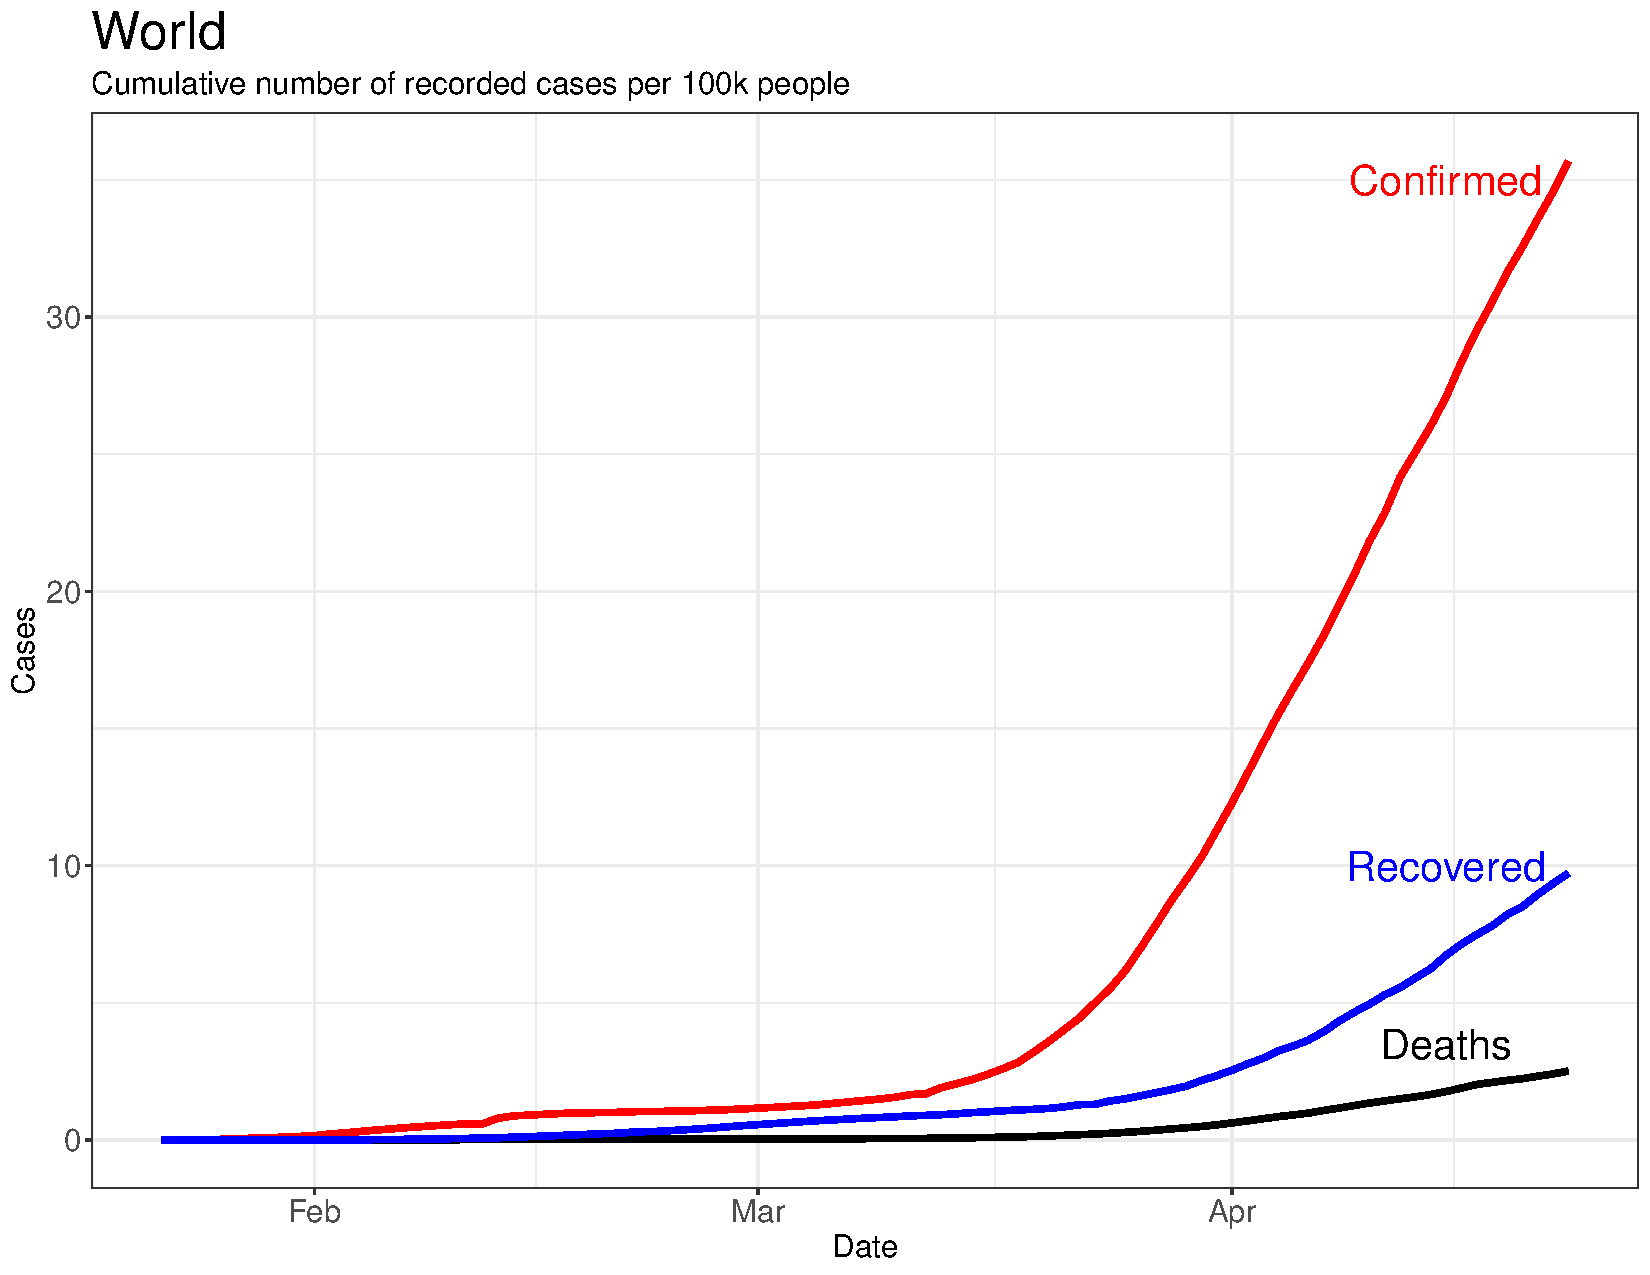
\includegraphics[width = 270pt]{Cases_world.pdf}
	\end{figure}
 \end{frame}

 \begin{frame}
 	\frametitle{COVID-19 weltweit}
		\centering
		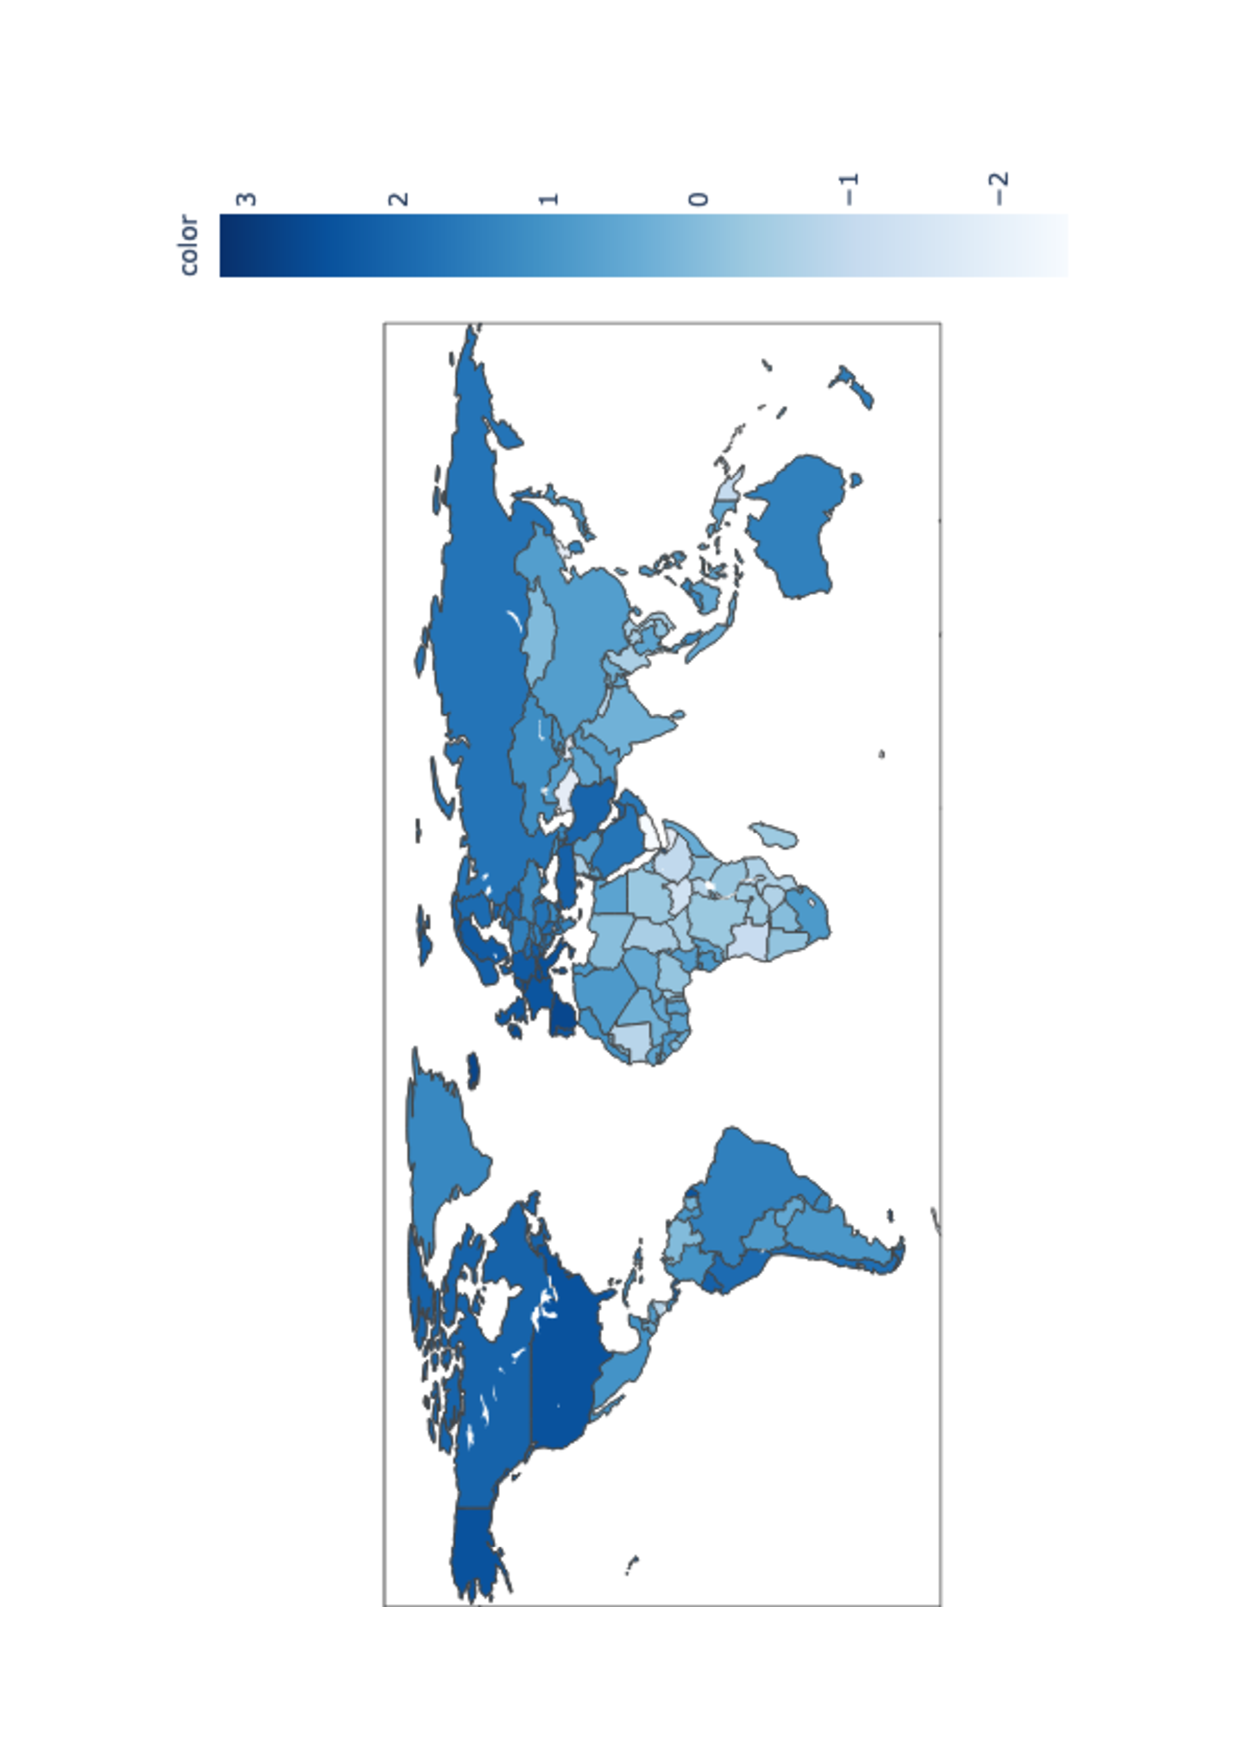
\includegraphics[width = 270pt, angle = -90]{map_confirmed.pdf}
 \end{frame}

 \begin{frame}
 	\frametitle{COVID-19 weltweit}
		\centering
		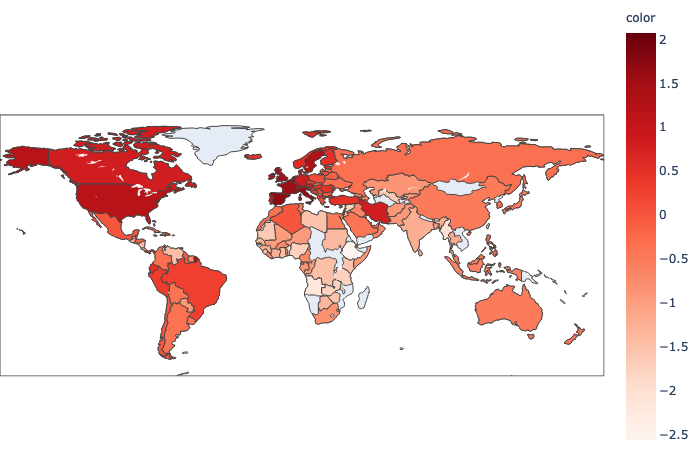
\includegraphics[width = 270pt, angle = -90]{map_death}
 \end{frame}
 
 \begin{frame}
 	\frametitle{COVID-19 weltweit bestätigte Fälle}
	\begin{figure}
		\centering
		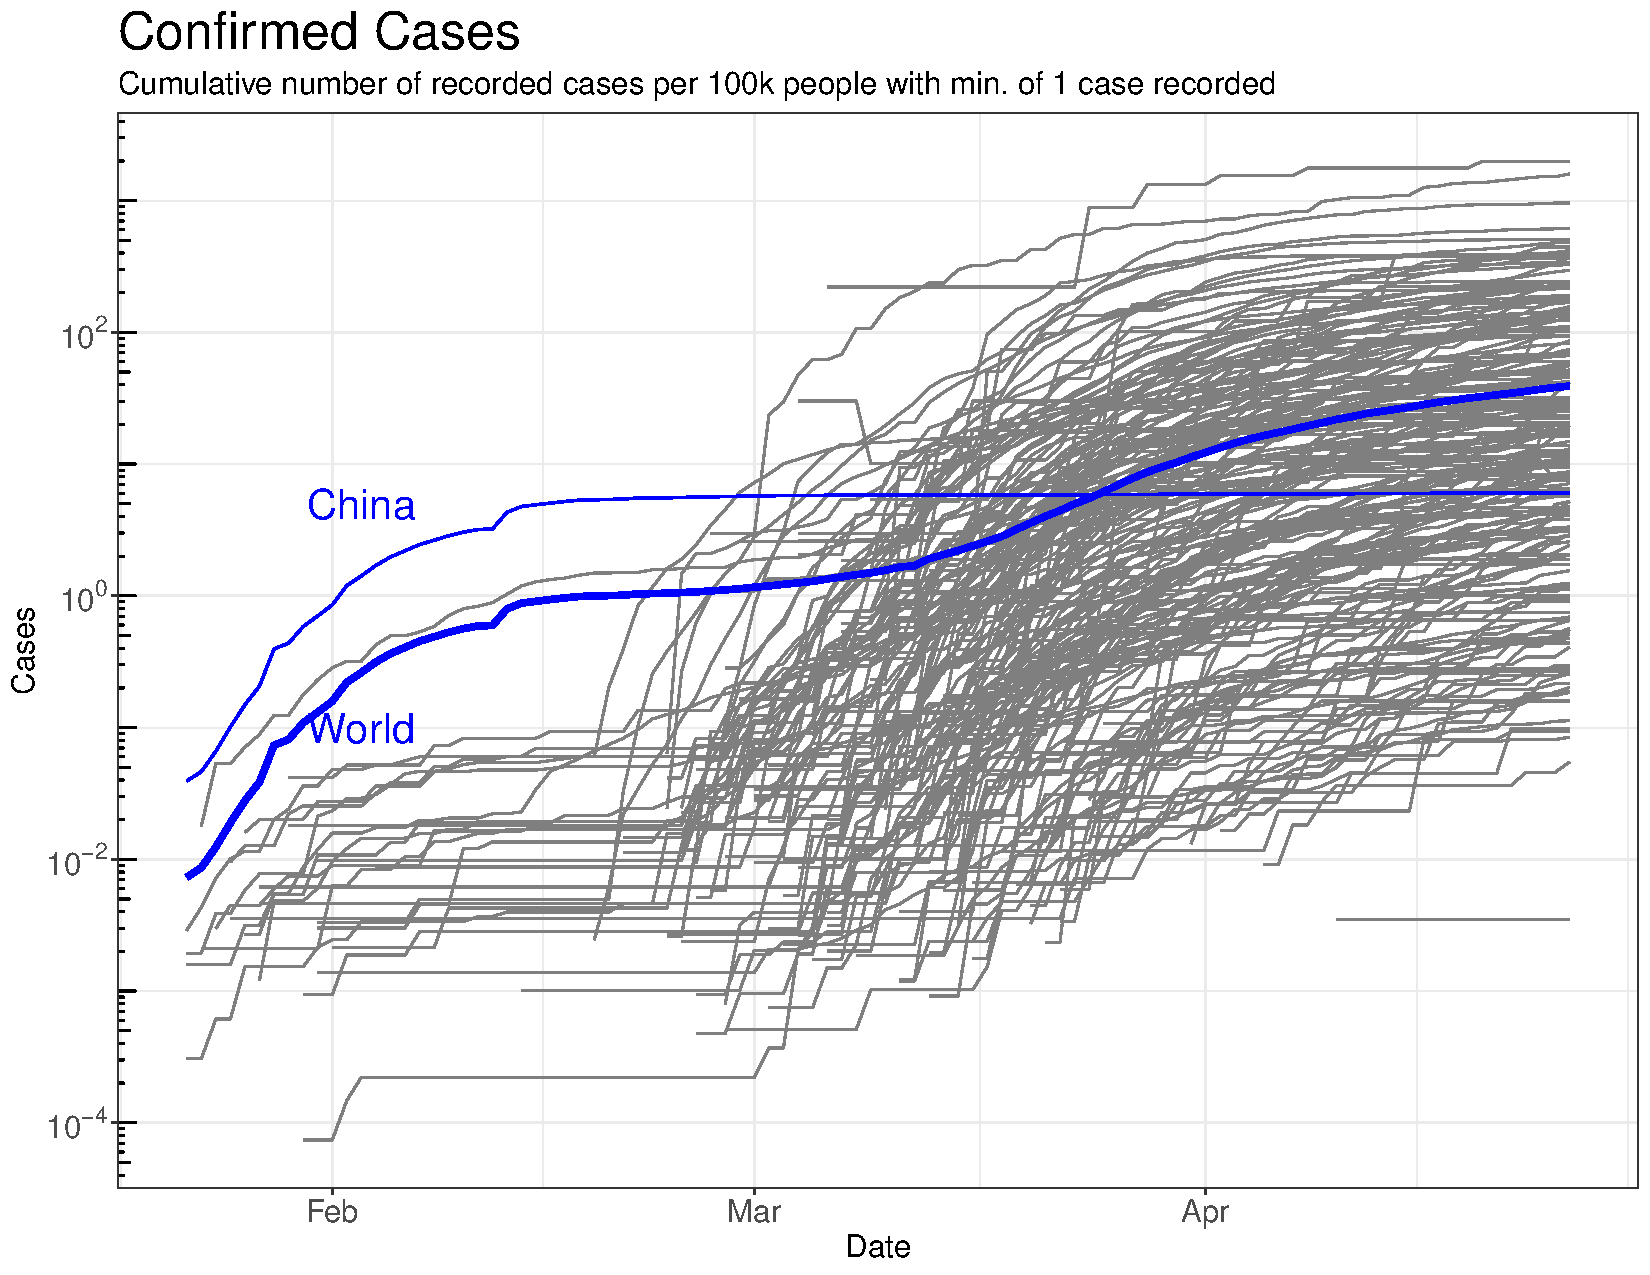
\includegraphics[width = 270pt]{Cases_cumulative_confirmed.pdf}
	\end{figure}
 \end{frame}

 \begin{frame}
 	\frametitle{COVID-19 weltweit bestätigte Todesfälle}
	\begin{figure}
		\centering
		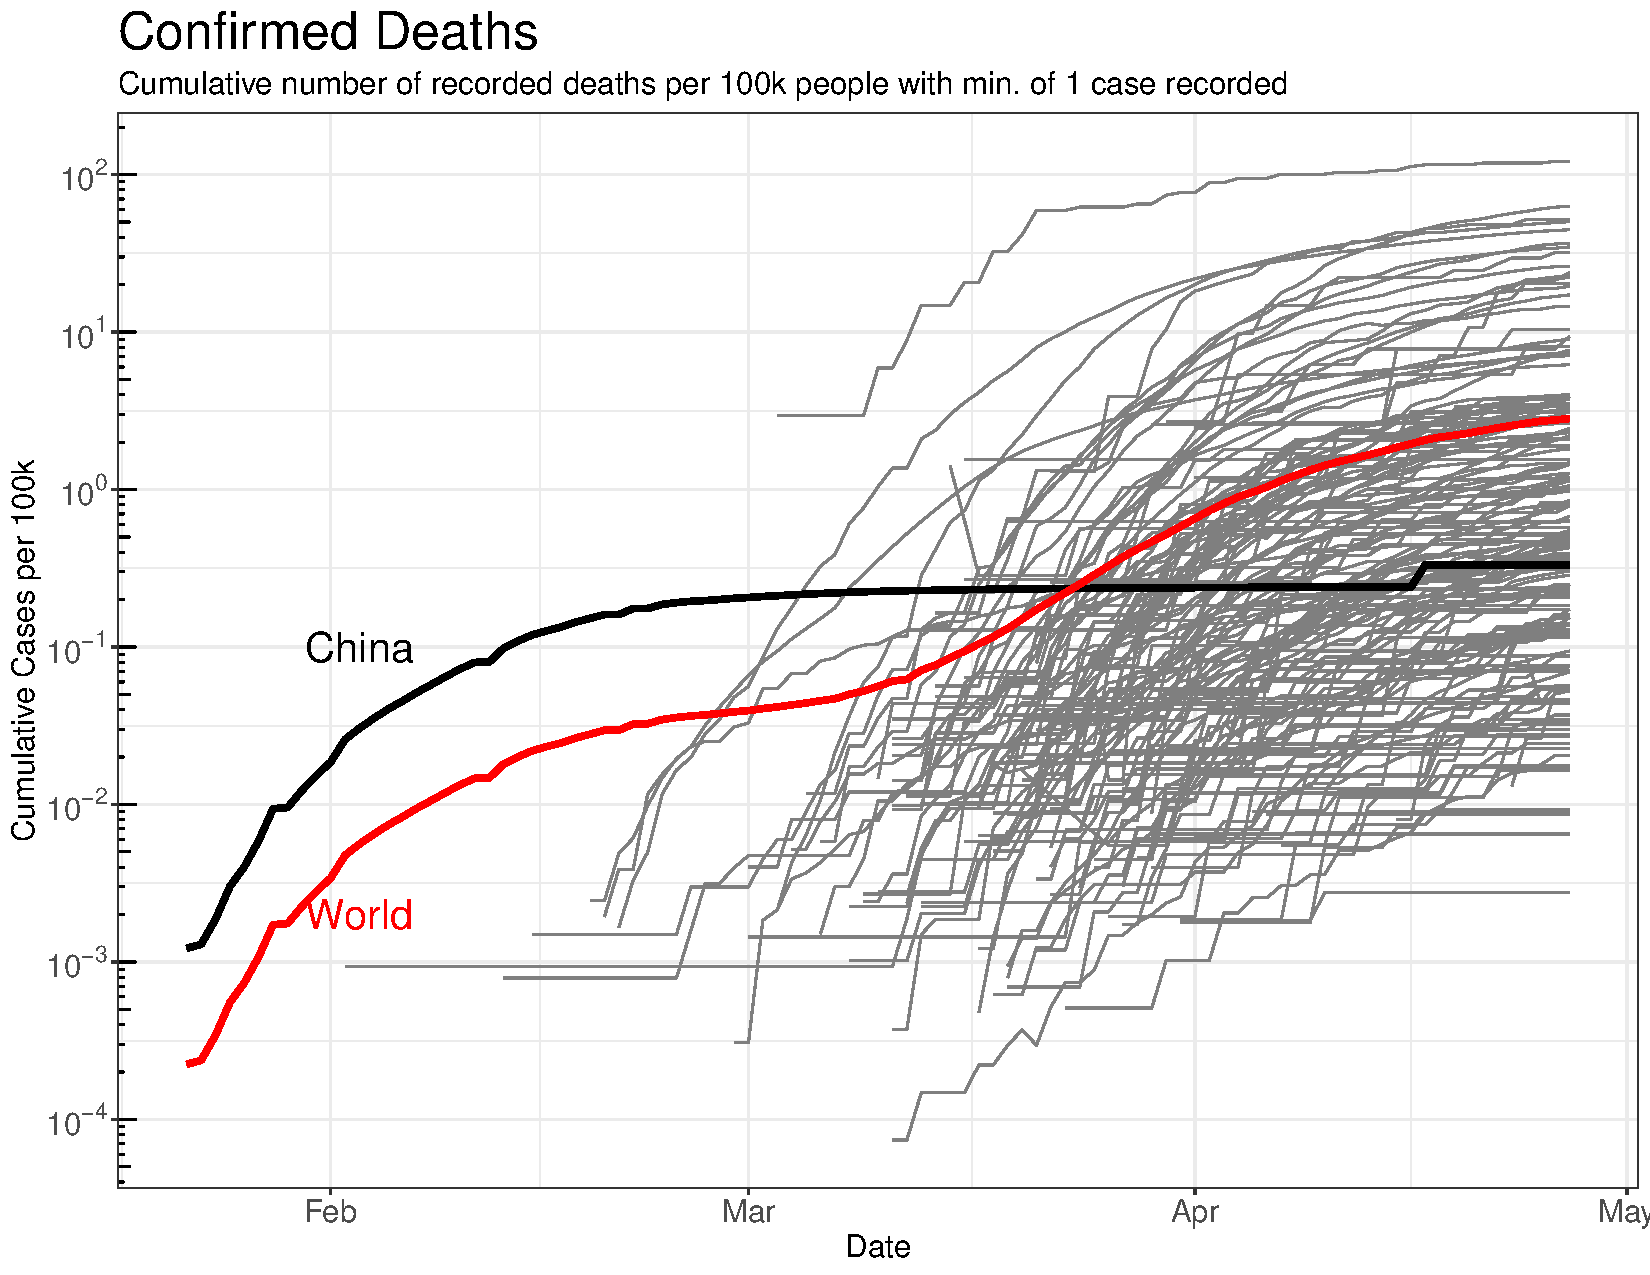
\includegraphics[width = 270pt]{Cases_cumulative_deaths.pdf}
	\end{figure}
 \end{frame}

 \begin{frame}
 	\frametitle{Zwischenergebnis}
 \end{frame}

\section{Wachstumsfaktoren der kumulativen Fälle und Todesfälle}
\begin{frame}
	\frametitle{Wiederholung: Wachstumsfaktor und geometrisches Mittel}
	\begin{boxeded}
		\textbf{Definition 1} \textit{Wachstumsfaktor}\\
		Sei $C_0, C_1, C_2, ...$ eine Zeitreihe von Fallzahlen zu den Zeitpunkten $0, 1, ..., n$. Dann ist für $i = 1, ..., n$ der i-te Wachstumsfactor $x_1$ gegeben durch $$ x_i = \frac{C_i}{C_{i-1}}.$$
	\end{boxeded}

	Die Fallzahlen $C_n$ zum Zeitpunkt $n$ sind gegeben durch $$C_n = C_0 \cdot x_1 \cdot x_2 \cdot ... \cdot x_n$$
\end{frame}

\begin{frame}
	\frametitle{Wiederholung: Wachstumsfaktor und geometrisches Mittel}
	\begin{boxeded}
		\textbf{Definition 2} \textit{Geometrisches Mittel}\\
		Das geometrische Mittel zu den Wachstumsfaktoren $x_1, x_2, ..., x_n$ ist gegeben durch $$\bar{x}_{geom} = (x_1 \cdot x_2 \cdot ... \cdot x_n)^{1/n}.$$ Daraus ergibt sich $C_n = C_0 \cdot x_1 \cdot x_2 \cdot ... \cdot x_n = C_0 \cdot (\bar{x}_{geom})^n$.
	\end{boxeded}
	\pause
	Wir betrachten im Folgenden den \emph{rolling geometric mean} der vergangenen 7 Tage. Dazu berechnen wir für jeden Zeitpunkt $i$ $$\bar{x}_{i, geom} = (x_i \cdot x_{i-1} \cdot x_{i-2} \cdot ... \cdot x_{i-6})^{1/7}.$$
\end{frame}

\begin{frame}
	\frametitle{Wachstumsfaktoren: Bestätigte Fälle}
	\begin{figure}
		\centering
		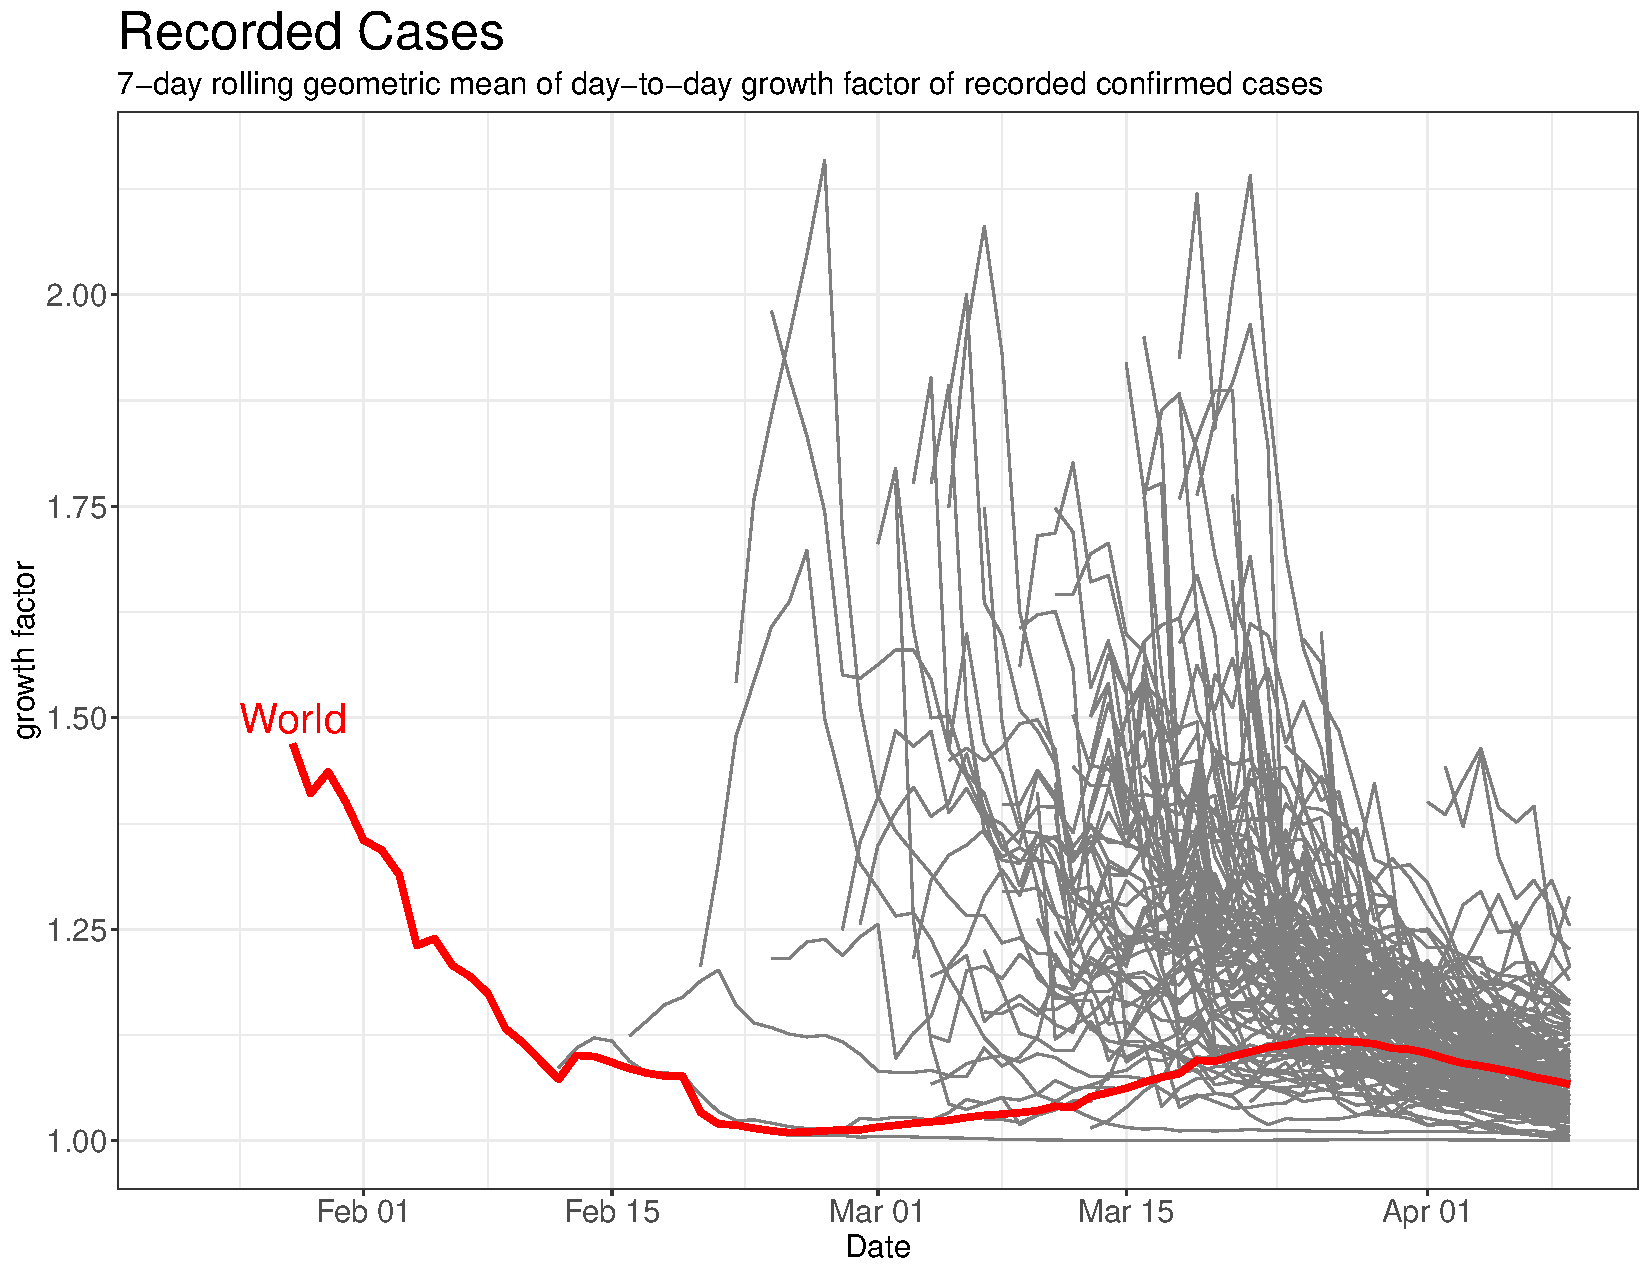
\includegraphics[width = 270pt]{GF_confirmed}
	\end{figure}
\end{frame}

\begin{frame}
	\frametitle{Wachstumsfaktoren: Todesfälle}
	\begin{figure}
		\centering
		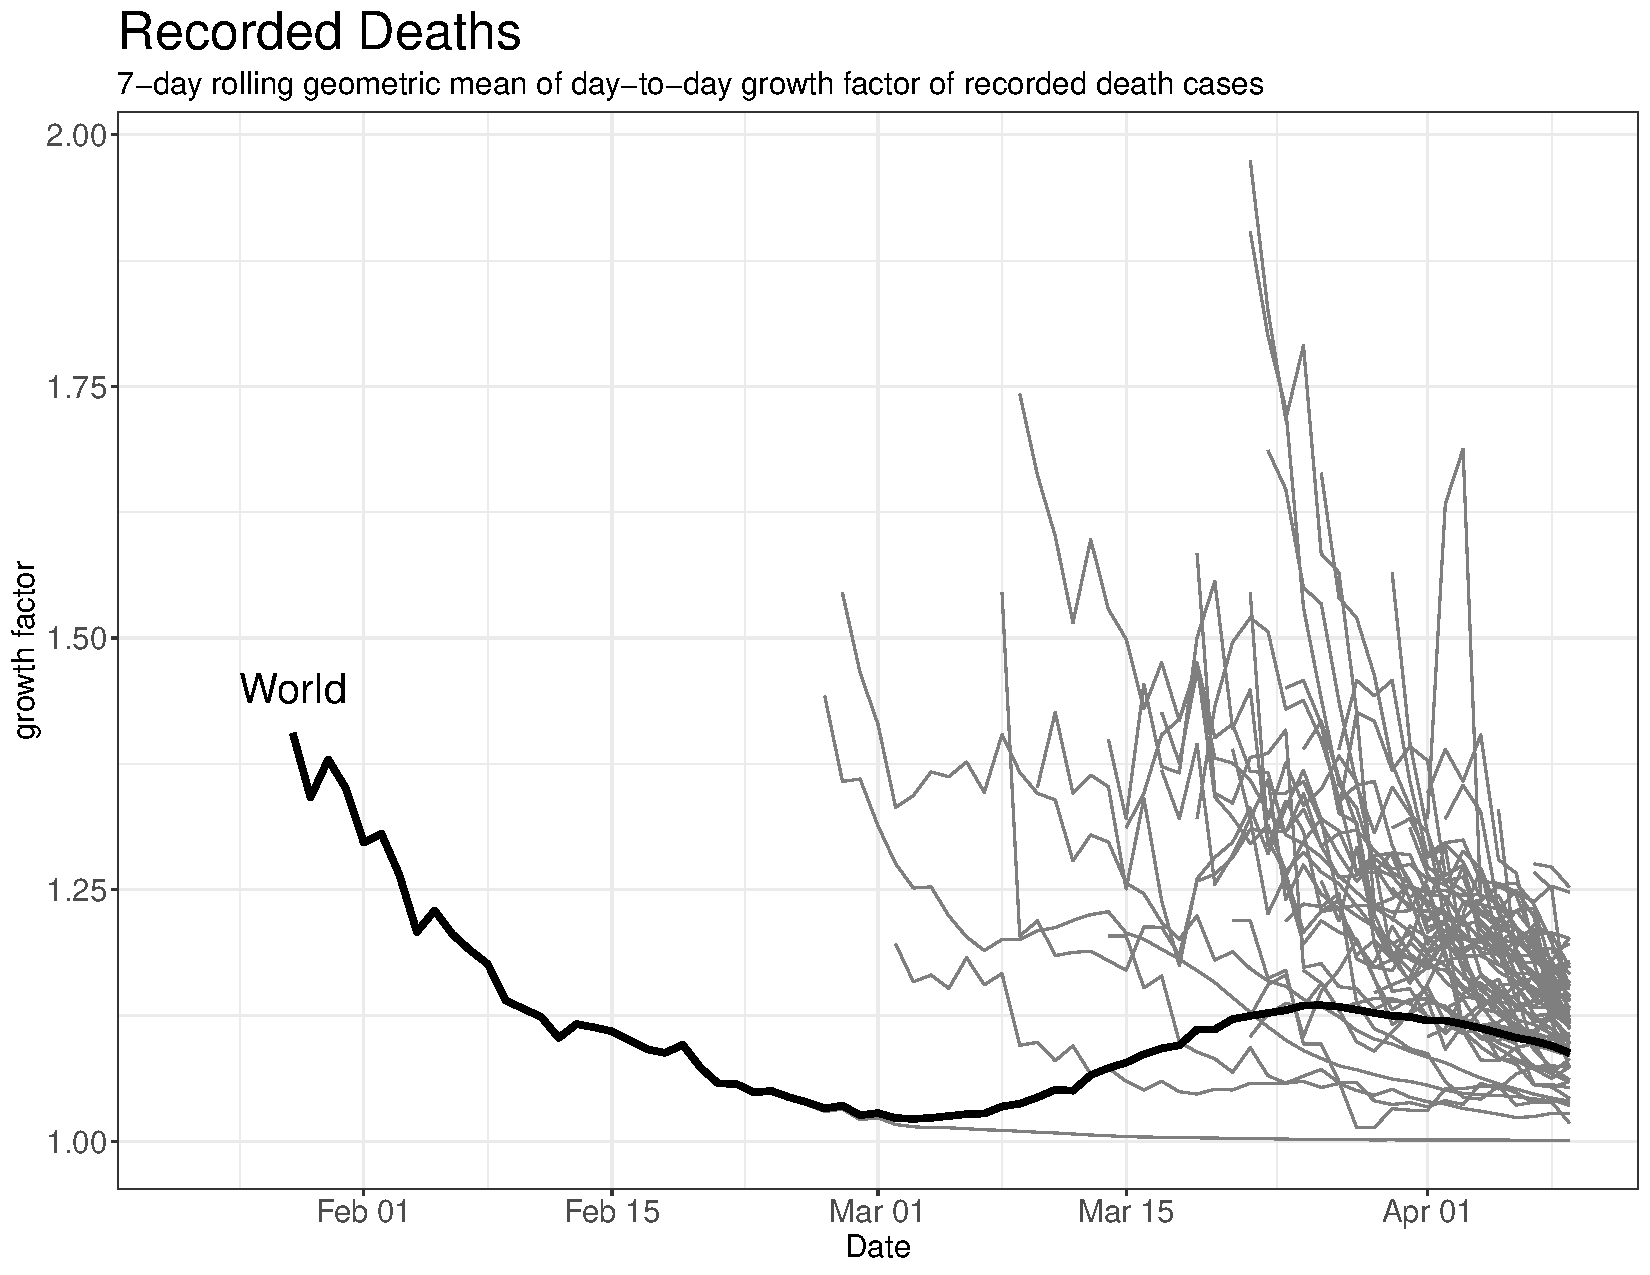
\includegraphics[width = 270pt]{GF_deaths}
	\end{figure}
\end{frame}

\begin{frame}
	\frametitle{Verdopplungszeit}
	Ausgehend von einem exponentielle Wachstum der Form $C_n = C_0 \cdot (\bar{x}_{n, geom})^{n}$ ergibt sie die "momentane" Verdopplunszeit $dt_i$ der Fallzahlen durch $$dt_i = \frac{ln(2)}{ln(\bar{x}_{i, geom})}.$$
	\pause
	\emph{Herleitung}: 
	\begin{align*} C_i \cdot (\bar{x}_{i, geom})^{dt_i} = 2 \cdot C_i 
		 &\iff (\bar{x}_{i, geom})^{dt_i} = 2 \\
	 	&\iff dt_i = \frac{ln(2)}{ln(\bar{x}_{i, geom})}.
	\end{align*}
\end{frame}

\begin{frame}
	\frametitle{Verdopplungszeit: Bestätigte Fälle}
	\begin{figure}
		\centering
		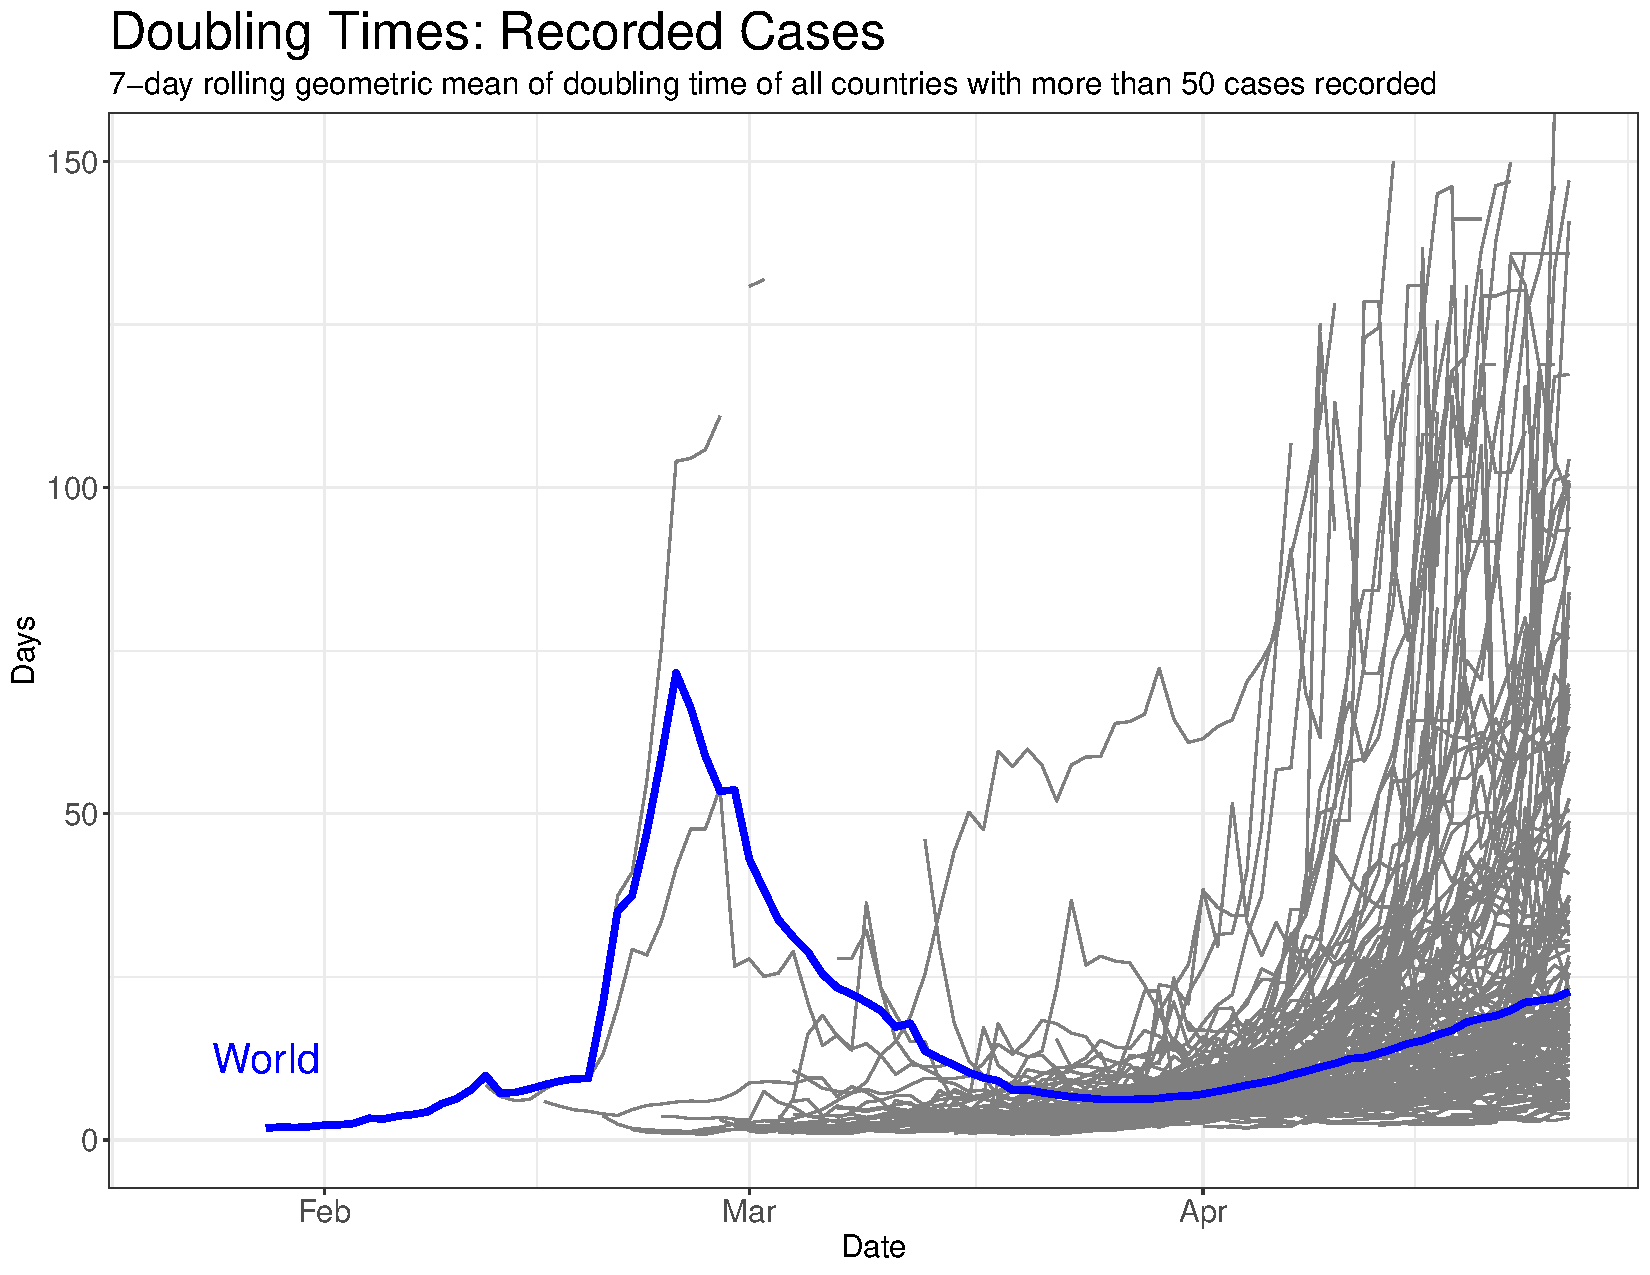
\includegraphics[width = 270pt]{DT_confirmed}
	\end{figure}
\end{frame}

\begin{frame}
	\frametitle{Verdopplungszeit: Todesfälle}
	\begin{figure}
		\centering
		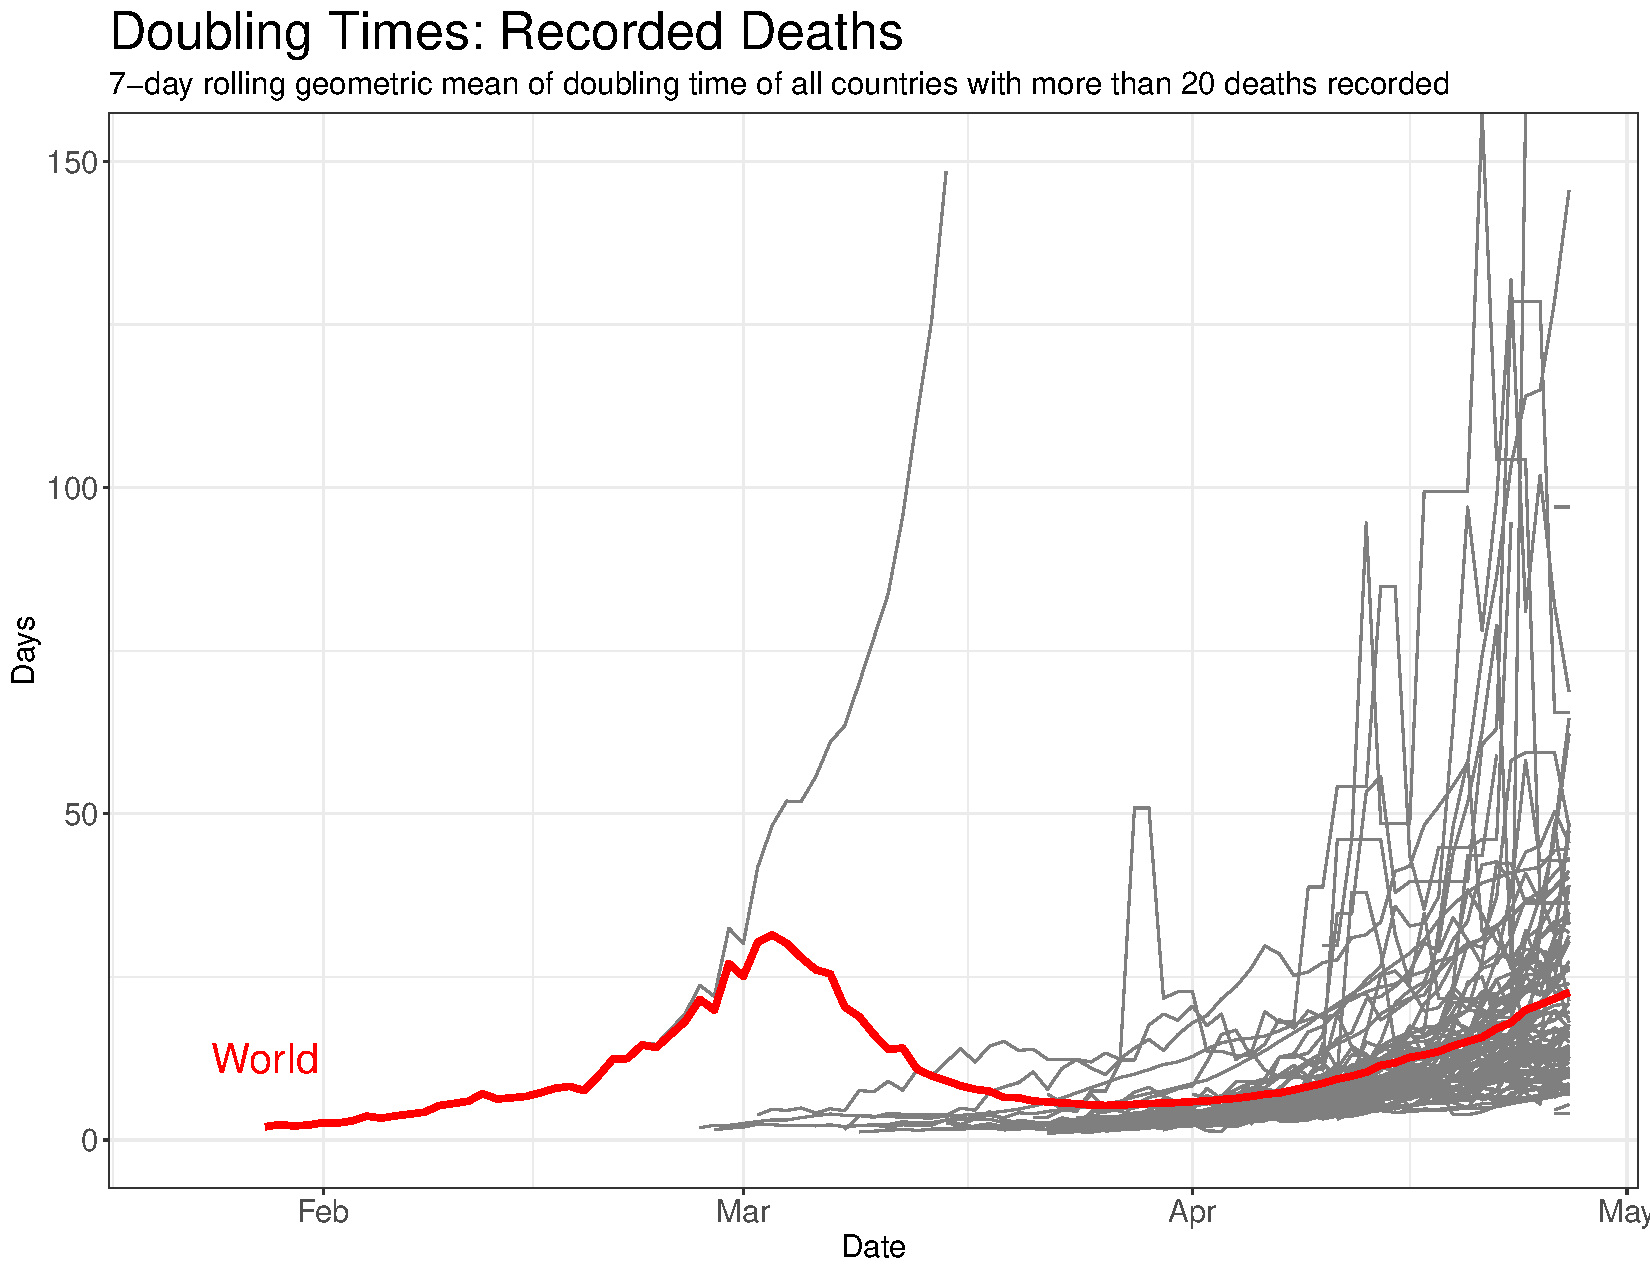
\includegraphics[width = 270pt]{DT_deaths}
	\end{figure}
\end{frame}

 \begin{frame}
 	\frametitle{Zwischenergebnis}
 \end{frame}

\section{Ländervergleich}
\begin{frame}
	\frametitle{Infektionsmaßnahmen}
	\centering
	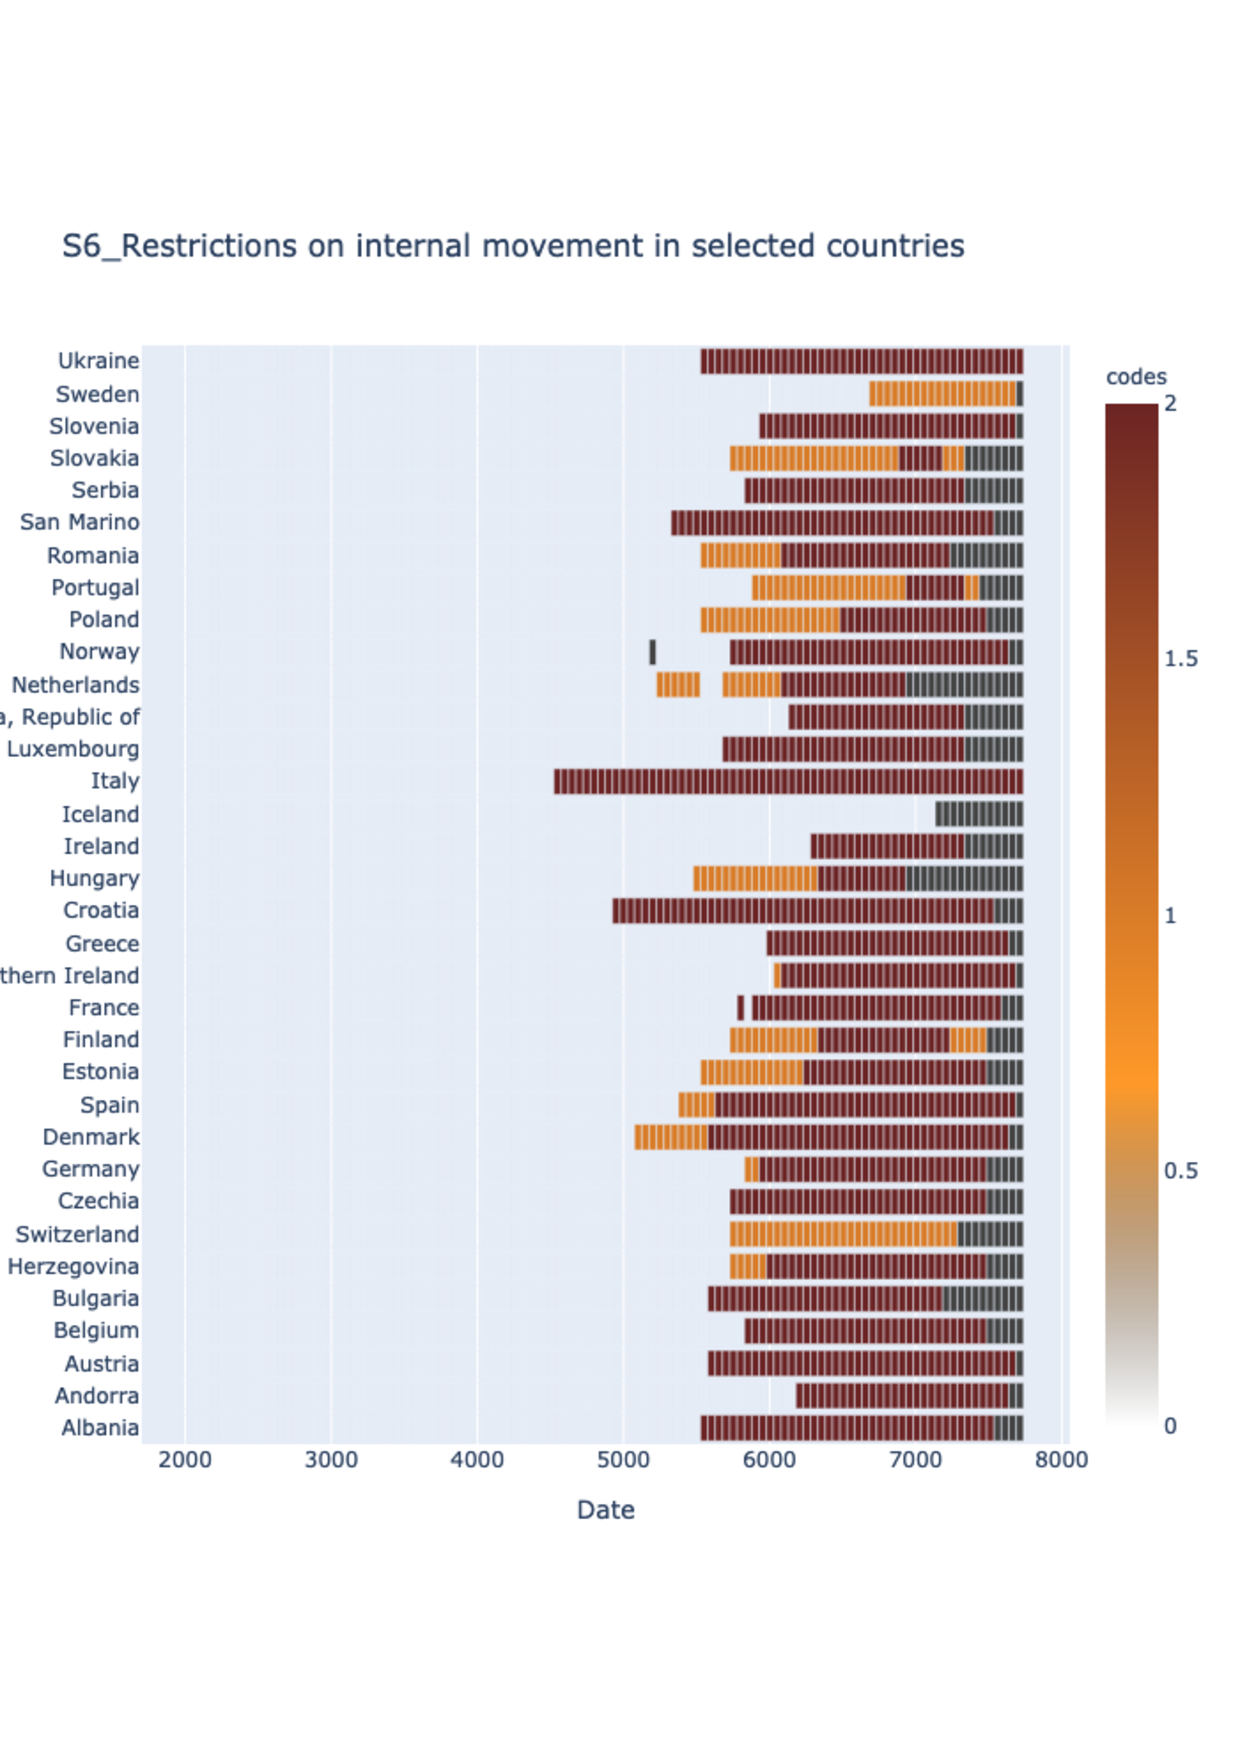
\includegraphics[width = 270pt]{responses_countries}
\end{frame}

\begin{frame}
	\frametitle{Diskussion}
	\begin{itemize}
		\item Die Berechnung des \emph{geometrischen Mittels der Wachstumsfaktoren} und der \emph{Verdopplungzeiten} beruhen auf der Annahme eines exponentielle Wachstums. Zulässigkeit?
		\item Starke Unterschiede in der Strenge der Ausgangsbeschränkungen einzelner Länder.
		\item Verschiedene Maßnahmen machen Gruppierung nur schwer möglich.
	\end{itemize}
\end{frame}
 
\end{document}